\section{Basics of Convex Analysis}
One of the stepping stones in the path toward understanding stochastic gradient descent is to first understand the usual deterministic gradient descent. Gradient descent is an algorithm that is part of a family of algorithms called descent methods which are mostly applicable to unconstrained minimization problems. The simplicity of unconstrained problems allows descent methods to be fast and easy to implement. When dealing with unconstrained problems, an important assumption is the convexity of the objective function. In \ref{eq:3} a definition is given. To understand convexity in general we need to understand the notions of affine sets and convex sets. Additionally, further definitions and regularity conditions require examination. These concepts are important because the convexity assumption plays a crucial role in the convergence properties of gradient descent. 
\subsection{Convexity}
\begin{definition}
Suppose $x_{1},x_{2} \in \mathbf{R}^{n}$ with $x_{1} \neq x_{2}$. Points of the form $y = \theta x_{1} + (1-\theta) x_{2},$ where $\theta \in \mathbf{R}$, form the $\textit{line}$ passing through $x_{1}$ and $x_{2}$. The parameter value $\theta = 0$ corresponds to $y = x_{2}$ and the value $\theta = 1$ corresponds to $y = x_{1}$. The set $[x_{1},x_{2}] = \{\theta x_{1} + (1-\theta) x_{2}: \theta \in [0,1]\}$ is called the (closed) \textit{line segment} between $x_{1}$ and $x_{2}$.
\end{definition}

\begin{definition}
(\cite[21]{boyd2004convex})
A set $C \subseteq \mathbf{R}^{n}$ is \textit{affine} if the line through any two distinct points in \textit{C} lies in \textit{C}, in other words, if for any $x_{1}, x_{2} \in C$ and $\theta \in \mathbf{R}$, we have $\theta x_{1} + (1-\theta) x_{2} \in C$.
\end{definition}

\begin{definition}
(\cite[23]{boyd2004convex})
A set \textit{C} is \textit{convex} if the line segment between any two points in \textit{C} lies in \textit{C}, In other words, if for any $x_{1}, x_{2}$ $\in C$ and any $\theta$ with $0 \leq \theta \leq 1$, we have $\theta x_{1} + (1-\theta) x_{2} \in C.$
\end{definition}
\vspace*{0pt}
\begin{figure}[h!]
    \centering
        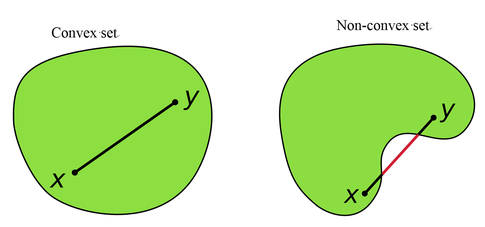
\includegraphics[width=0.45\textwidth]{Pictures/Convex ex.png}
    \caption{Example of a convex and non-convex set}
    \label{fig:conv-nonconv}
\end{figure}

\begin{definition}
(\cite[36]{boyd2004convex})
A function $f: \mathbf{R}^{n} \longrightarrow \mathbf{R}^m$ is \textit{affine} if it is a sum of a linear function and a constant, in other words, if it has a form $f(x) = Ax + b$, where $A \in \mathbf{R}^{m \times n}$ and $b \in \mathbf{R}^m$.
\end{definition}

\begin{definition}\label{definition.2.4}
(\cite[67]{boyd2004convex})
A function $f: \mathbf{R}^{n} \longrightarrow \mathbf{R}$ is convex if $\textbf{dom}(f)$ is a convex set and if for all $x,y \in \textbf{dom} \textit{f}$, and with $0 \leq \theta \leq 1$, we have 
\begin{equation*}\label{eq:4}\tag{2.1.1}
\begin{aligned}
    &f(\theta x + (1-\theta) y) \leq \theta f(x) + (1-\theta) f(y)
\end{aligned}
\end{equation*}
\end{definition}

\begin{proposition}\label{compaf}
(\cite[79]{boyd2004convex})
Suppose $f: \mathbf{R}^{n} \longrightarrow \mathbf{R}, A \in \mathbf{R}^{n\times m},$ and $b \in \mathbf{R}^{n}.$ Define $g: \mathbf{R}^{m} \longrightarrow \mathbf{R}$ by $$g(x)=f(Ax+b),$$ with $\textbf{dom} g = \{x\text{ }|\text{ }Ax+b \in \textbf{dom} (f)\}.$ Then if $f$ is convex, so is $g$.
\end{proposition}
\begin{proof}
Suppose that $f$ is convex. To show: $g$ is convex. Let $x,y \in \mathbf{R}^{n}$ and fix $\theta \in [0,1].$ Then
\begin{align*}
g(\theta x + (1-\theta)y) &= f(A(\theta x + (1-\theta)y) + b)\\
&= f(\theta(Ax - Ay) + Ay + b)\\
&= f(\theta(Ax + b) + (1 - \theta)(Ay+b))\\
&\leq \theta f(Ax + b) + (1-\theta) f(Ay + b)\\
&= \theta g(x) + (1-\theta)g(y).
\end{align*}
$x,y$ and $\theta$ are arbitrarily fixed. So the inequality holds $\forall \text{ } x,y \in \mathbf{R}^{n}$ and $\theta \in [0.1].$ Hence, $g$ is convex. 
\end{proof}
\subsection{Gradient and Optimality}
\begin{definition}[Gradient]\label{gradient}
If $f$ is differentiable along each axis, we denote 
\begin{equation*}\tag{2.2.1}
\begin{aligned}
    &\nabla f(x) \overset{def.}{=} \left(\frac{\partial f(x)}{\partial x_{1}},\ldots,\frac{\partial f(x)}{\partial x_{d}}\right)^{T} \in \mathbf{R}^{n}
\end{aligned}
\end{equation*}
the gradient vector, so that $\nabla f: \mathbf{R}^{n}\longrightarrow \mathbf{R}^{n}$ is a vector field.
\end{definition}

\begin{lemma}[First-order conditions]\label{lemma.2.1}
\textnormal{(\cite[69]{boyd2004convex})}
Suppose \textit{f} is differentiable. In other words, $\nabla f$ exists at each point in $\textbf{dom} (f)$. Then \textit{f} is convex if and only if $\textbf{dom} (f)$ is convex and
\begin{equation*}\label{eq:5}\tag{2.2.2}
\begin{aligned}
    &f(y) \geq f(x) + \nabla f(x)^{T}(y-x)
\end{aligned}
\end{equation*}
holds for all $x,y \in \textbf{dom} (f)$. This inequality is illustrated in \ref{eq:5}
\end{lemma}
The affine function $y \mapsto f(x) + \nabla f(x)^{T}(y-x)$ is, of course, the first-order Taylor approximation of $f$ near $x$. Lemma \ref{lemma.2.1} contains an if and only if statement which states that for convex functions, the first-order Taylor approximation is always a \textit{global under estimator} for the function and that the converse is also true. In the context of optimization, finding the minimum value of a function requires identifying the point at which the function attains its lowest value. Setting the gradient to zero serves as a means of locating an optimal solution, a point of inflection where the rate of change of the function is zero and the function is neither increasing nor decreasing. 
\begin{proposition}\label{eq:local_conv}
\textnormal{(\cite[7]{coursenotesML})}
If $f$ attains a local minimum at $x^{*}$ (i.e. that $f(x^{*}) \leq f(x) $ for all $x$ in some ball around $x^{*}$) then $$\nabla f(x^{*}) = 0.$$
\end{proposition}
\begin{proof}
One has for $\epsilon$ small enough and $u$ fixed
$$f(x^{*}) \leq f(x^{*} + \epsilon u) = f(x^{*}) + \epsilon \langle \nabla f(x^{*}),\text{ }u\rangle + o(\epsilon) \implies \langle \nabla f(x^{*}),\text{ }u\rangle \geq o(1) \implies \langle \nabla f(x^{*}),\text{ }u\rangle \geq 0.$$ So applying this for $u$ and $-u$ in the previous equation shows that $\langle \nabla f(x^{*}),\text{ }u\rangle = 0$ for all $u$, and hence $\nabla f(x^{*}) = 0.$
\end{proof}
\begin{proposition}\label{eq:argmin_conv}
\textnormal{(\cite[7]{coursenotesML})}
If $f$ is convex and attains a local minimum at $x^{*}$, then this local minimum is also a global minimum. If $f$ is differentiable and convex, $$x^{*} \in \underset{x}{\textnormal{argmin}}f(x) \iff \nabla f(x^{*}) = 0.$$
\end{proposition}
\begin{proof}
Let $x \in \mathbf{R}^n$ be fixed. Then there exists $0 < \theta < 1$ small enough such that $\theta x + (1-\theta)x^{*}$ is close enough to $x^{*},$ and so since it is a local minimizer $$f(x^{*}) \leq f(\theta x + (1-\theta)x^{*}) \leq \theta f(x) + (1-\theta) f(x^{*}) \implies f(x^{*}) \leq f(x).$$ Now $x \in \mathbf{R}^n$ is fixed, so this is true $\forall x \in \mathbf{R}^n$, thus $x^{*}$ is a global minimum. For the second part, the '$\Rightarrow$' implication is proven in proposition \ref{eq:local_conv}. Suppose that $\nabla f(x^{*}).$ Since the graph of $x$ is above its tangent by convexity (as stated in lemma \ref{lemma.2.1}), 
\begin{equation*}
f(x) \geq f(x^{*}) + \langle \nabla f(x^{*}),\text{ }x - x^{*}\rangle = f(x^{*})
\end{equation*}
\end{proof}
The last inequality shows that $x^{*}$ is a global minimizer of the function $f$. Hence, if \textit{f} is differentiable and convex, a necessary and sufficient condition for a point $x^{*}$ to be optimal is given by: $\nabla f(x^{*}) = 0.$ One can strengthen the convexity condition from Definition \ref{definition.2.4} and impose that the inequality is strict for $\theta \in [0,1].$ In this case $f$ is called strictly convex and $x^{*}$ is unique. Lemma \ref{lemma.2.1} will especially prove to be useful in the convergence analysis of descent methods. In many situations neither Definition \ref{definition.2.4} nor the first-order conditions are used to check the convexity of a function. For this, we need additional tools which consist of several conditions that are called second-order conditions. For this, we need the notions of the Hessian and positive semidefiniteness. 

\begin{definition}[Hessian]
(\cite[748]{adams2013calculus})
Suppose $f: \mathbf{R}^{n} \longrightarrow \mathbf{R}$ is a function such that $x\mapsto f(x)$ with the property that all second-order partial derivatives of $f$ exist, then the Hessian matrix $\mathcal{H}$ of $f$ is an $n \times n$ matrix and is given by:
\begin{equation*}
\mathcal{H}(x) = 
\begin{bmatrix}
f_{11}(x) & f_{12}(x) & \cdots & f_{1d}(x) \\
f_{21}(x) & f_{22}(x) & \cdots & f_{2d}(x) \\
\vdots             & \vdots             & \ddots & \vdots             \\
f_{d1}(x) & f_{d2}(x) & \cdots & f_{dd}(x)
\end{bmatrix}
\end{equation*}
where $f_{ij} = \frac{\partial^{2}f}{\partial x_{i}\partial x_{j}}$
\end{definition}

\begin{definition}[Positive semidefiniteness]\label{posdef}
(\cite{doi:https://doi.org/10.1002/9780470173862.app3})
Suppose that $\mathcal{V}$ is an $n \times n$ symmetric matrix, i.e., $\mathcal{V}=\mathcal{V}^{T}$, then $\mathcal{V}$ is said to be positive semidefinite if 
\begin{equation*}\label{eq:6}\tag{2.2.3}
\begin{aligned}
    &x^{T} \mathcal{V} x \geq 0 
\end{aligned}
\end{equation*}
for all $x \in \mathbf{R}^{n}$. Notation: $\mathcal{V} \succeq 0.$
\end{definition}
\begin{lemma}[Second-order conditions]\label{second-ord-cond}
(\cite[71]{boyd2004convex})
We now assume that f is twice differentiable, that is, its Hessian or second derivative $\nabla^{2}f$ exists at each point in $\textbf{dom} (f)$. Then f is convex if and only if $\textbf{dom} (f)$ is convex and its Hessian is positive semidefinite: for all $x \in \textbf{dom} (f),$ 
\begin{equation*}\label{eq:9}\tag{2.2.4}
\begin{aligned}
    &\nabla^{2}f(x) \succeq 0.
\end{aligned}
\end{equation*}
\end{lemma}
\begin{proof}
    
\end{proof}

\newpage
\subsection{Unconstrained Minimization Problems}
In this section unconstrained minimization problems will be discussed in more detail. Descent methods play a big role in solving these problems. Descent methods are optimization algorithms for solving the unconstrained minimization problem 
\begin{equation*}\label{eq:8}\tag{2.3.1}
\begin{aligned}
    &\text{minimize} \text{ } f(x)\\ 
    &\textbf{dom} (f) = \mathbf{R}^n
\end{aligned}
\end{equation*}
where $f: \mathbf{R}^{n} \longrightarrow \mathbf{R}$ is the objective function. The true optimal solution to this problem may be a set of $x^{*} \in D$ of all optimal points in $D$, rather than a single minimum. In general, there might be no solution to the optimization \eqref{eq:8}. This is the case if $f$ is unbounded below, for example, if $f(x) = -x^{2}$ in which case the minimum value is $-\infty.$ It can also be the case that $f$ does not grow at infinity, for example if $f(x) = e^{-x}$, for which min$f$ = 0, but there is no minimizer. The task of any good optimization problem is to find globally optimal solutions if they exist. The objective function could be continuous, discontinuous, linear, non-linear, and convex. Problems with convex objectives are easiest to work with, since in that case, the problem is solvable and optimal solutions in which the function attains the global minimum can be found. The best case scenario is when there is one unique optimal solution $x^{*}$. For convex functions, solving the unconstrained minimization problem is the same as finding a solution to \eqref{eq:argmin_conv}. Since there are $d$ variables $(x_{1},\ldots,x_{d}),$ a system of $d$ equations needs to be solved. This can be a difficult process to solve analytically, especially in the case of non-linear functions and when $d$ is large. Therefore, usually, iterative algorithms are consulted. Such an algorithm computes a sequence of points called a minimizing sequence for \ref{eq:8}. First a starting point $x^{(0)}$ is chosen and in the following iterations the algorithm computes $x^{(1)}, x^{(2)},\ldots$ such that $f(x^{(k)}) \longrightarrow p^{*}=f(x^{*})$ as $k \longrightarrow \infty$. The key consideration when selecting $x^{(0)}$ is addressed by the following definition:
\begin{definition}[Sublevel sets]
\cite[75]{boyd2004convex}  
The $\alpha-\textit{sublevel set}$ of a function $f: \mathbf{R}^{n} \longrightarrow \mathbf{R}$ is defined as $$C_{\alpha} = \{x \in \textbf{dom} (f) \text{ }|\text{ } f(x) \leq \alpha\}.$$
\end{definition}
\begin{remark}
\cite[75]{boyd2004convex}  
Sublevel sets of a convex function are convex, for any value of $\alpha$.
\end{remark}
\begin{proof}
Suppose that the function $f$ is convex. Let $x,y \in C_{\alpha}$ and fix $\theta \in [0,1]$. Then $$f(\theta x + (1-\theta)y) \leq \theta f(x) + (1-\theta)f(y) \leq \theta \alpha + (1-\theta)\alpha = \alpha$$
Since $x,y$ and $\theta$ are arbitrarily chosen, the statement holds for all $x,y \in C_{\alpha}$ and $\theta \in [0,1]$.
\end{proof} 
Now trivially it is required that $x^{(0)} \in \textbf{dom} (f)$, and as discussed in \cite[457]{boyd2004convex} the sublevel set 
\begin{equation*}\label{eq:13}\tag{2.3.2}
\begin{aligned}
    &S = \{x \in \textbf{dom} (f) \text{ }|\text{ } f(x) \leq f(x^{0})\}
\end{aligned}
\end{equation*}
must be closed. This condition is satisfied for all $x^{(0)} \in \textbf{dom} (f)$ if the function $f$ is closed. We call $f$ closed if all its sublevel sets are closed. Continuous functions with $\textbf{dom} (f) = \mathbf{R}^{n}$ are closed, so if $\textbf{dom} (f) = \mathbf{R}^{n}$, the initial sublevel set condition \ref{eq:13} is satisfied by any $x^{(0)}$. In this thesis, most of the functions that are examined are continuous functions on $\mathbf{R}^{n}.$ Hence, we have the freedom to choose any particular $x^{(0)}$ as a starting point. Iterative algorithms that solve problem \eqref{eq:8} terminate whenever $f(x^{(k)}) - p^{*} \leq \epsilon$ for some tolerance $\epsilon$ small and $k \in \mathbb{N}$.








